\documentclass{article}%
\usepackage[T1]{fontenc}%
\usepackage[utf8]{inputenc}%
\usepackage{lmodern}%
\usepackage{textcomp}%
\usepackage{lastpage}%
\usepackage{authblk}%
\usepackage{graphicx}%
%
\title{Expression of Mina53, a novel c{-}Myc target gene, is a favorable prognostic marker in early stage lung cancer}%
\author{Ariel Simmons}%
\affil{CAS Key Laboratory of Pathogenic Microbiology and Immunology, Institute of Microbiology, Chinese Academy of Sciences, Beijing, China}%
\date{01{-}01{-}2012}%
%
\begin{document}%
\normalsize%
\maketitle%
\section{Abstract}%
\label{sec:Abstract}%
What can you do to stem the cancerous stem cells that have developed from your tumor?\newline%
It is known that a certain cancer{-}fighting protein called PAR3 is often involved in pathways in the tumor that cause cancer and may have been found to contribute to an increased risk of breast cancer. Now, one expert says the cancer has grown tumors in two types of mice  the muno tumor and the buno tumor.\newline%
Scientists at the Harvard Medical School tested the protein KSA by adding it to certain breast cancer drugs while blocking an important tumor{-}promoting protein called epidermal growth factor receptor (EGFR). The analysis shows that in both MUC and BBRM, the PAR3 protein was activated by EGFR and helped the tumors stage{-}out to meet the EGFR{-}chosen target of the chemotherapy drugs.\newline%
The researchers say this is the first time PAR3 has been used in an uncontrolled, human trial.

%
\subsection{Image Analysis}%
\label{subsec:ImageAnalysis}%


\begin{figure}[h!]%
\centering%
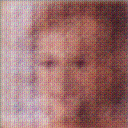
\includegraphics[width=150px]{500_fake_images/samples_5_282.png}%
\caption{A Close Up Of A Person Holding A Toothbrush}%
\end{figure}

%
\end{document}